\documentclass{article}

% If you do not have the 'neurips_2019' package specifically, 
% you can often use 'preprint' or standard article formatting. 
% Assuming the user has the style file provided in the prompt context:
\usepackage[final]{neurips_2019}

\usepackage[utf8]{inputenc}
\usepackage[T1]{fontenc}
\usepackage{hyperref}
\usepackage{url}
\usepackage{booktabs}
\usepackage{amsfonts}
\usepackage{nicefrac}
\usepackage{microtype}
\usepackage{graphicx}
\usepackage{xcolor}
\usepackage{amsmath} % Added for math environments
\usepackage{subcaption}
\usepackage{siunitx}
\usepackage{booktabs}  % for \toprule, \midrule, \bottomrule
\usepackage{multirow}  % for \multirow
\usepackage{tikz}
\usetikzlibrary{shapes,arrows,positioning,calc,fit}

\title{
  Active Characterization of Non-Cooperative Resident Space Objects Using Reinforcement Learning \\
  \vspace{1em}
  \small{\normalfont Stanford AA228 Project} 
}

\vspace{-40pt}

\author{
  Rahul Ayanampudi \\
  Department of Aeronautics and Astronautics \\
  Stanford University \\
  \texttt{rayanam@stanford.edu} \\
  \And
  Sebastian Martinez \\
  Department of Aeronautics and Astronautics \\
  Stanford University \\
  \texttt{sebasmp@stanford.edu}
}

\begin{document}
\maketitle
\begin{abstract}
Future missions for in-orbit servicing and active debris removal require autonomous spacecraft to characterize non-cooperative Resident Space Objects (RSOs) prior to proximity operations. This paper presents a reinforcement learning framework for active characterization, enabling a servicer spacecraft to autonomously plan maneuvers that maximize information gain regarding a target's 3D shape. We formulate the problem as a Partially Observable Markov Decision Process (POMDP) where the agent maintains a probabilistic voxel grid belief of the target. We implement a custom orbital dynamics simulator with Monte Carlo Tree Search (MCTS) as a classical planning baseline and develop an AlphaZero-inspired neural network that learns to approximate MCTS planning through self-play. Our results demonstrate that AlphaZero MCTS achieves superior performance over pure MCTS, reducing belief entropy by 97.1\% with only 0.11 m/s fuel expenditure compared to pure MCTS which achieves 96.77\% reduction with 0.31 m/s. The AlphaZero agent executes 65\% less fuel and 57\% fewer maneuvers while achieving better reconstruction quality, validating the approach for fuel-efficient autonomous shape reconstruction in Low Earth Orbit (LEO) environments.
\end{abstract}

\section{Introduction}
The proliferation of space debris and the growing need for on-orbit servicing have made the autonomous characterization of Resident Space Objects (RSOs) a critical capability for future space missions. Before a servicer spacecraft can safely attempt docking or debris removal, it must fully characterize the target, a process that involves determining the relative orbit and reconstructing the target's 3D shape \citep{kruger2024adaptive}. Current observer systems largely rely on passive sensing, which suffers from range ambiguities and slow convergence rates due to a lack of geometric diversity in viewing angles.

To overcome these limitations, we propose an active sensing framework where the agent explicitly decides on maneuvers ($\Delta v$) to acquire the most informative observations. This problem presents significant challenges in several domains: orbital mechanics, guidance, navigation, and control (GNC), and computer vision. Furthermore, maneuvers that are optimal for orbit determination, such as those inducing parallax, are not necessarily optimal for shape reconstruction, which requires a diverse set of viewing angles to resolve occlusions. 

We model this problem as a POMDP. The input to our algorithm includes the fully observable physical state of the servicer relative to the target and the agent's internal belief state regarding the target's shape. The output is a discrete action representing an impulsive maneuver in the Radial-Tangential-Normal (RTN) frame. Training a policy that balances the cost of fuel expenditure against the information gain derived from reducing uncertainty in the target's volumetric model is done by leveraging an AlphaZero-style reinforcement learning architecture.

The discrete action space problem formulation offers some advantages. First, impulsive spacecraft maneuvers naturally correspond to discrete actions, as thrusters execute finite-duration burns modeled as instantaneous velocity changes. Second, tree search can systematically evaluate possible maneuvers at each decision point \citep{kocsis2006bandit}, enabling principled long-horizon planning. This is critical for active sensing, where the information gain of future observations depends on selecting the right sequence of maneuvers.

The remainder of this paper is organized as follows: Section \ref{sec:related} reviews related work in autonomous spacecraft navigation and reinforcement learning. Section \ref{sec:dataset} describes the simulation environment and POMDP formulation. Section \ref{sec:methods} presents the MCTS baseline and AlphaZero training framework. Section \ref{sec:results} reports experimental results comparing pure MCTS and AlphaZero performance. Section \ref{sec:conclusion} concludes with future work directions.

\section{Related Work}
\label{sec:related}
The challenge of autonomous spacecraft navigation has been extensively studied in the context of cooperative rendezvous. However, non-cooperative proximity operations introduce high uncertainty. \citet{kruger2024adaptive} proposed an adaptive end-to-end architecture for autonomous navigation, highlighting the necessity of robust estimation filters for proximity operations. Building on this, \citet{kruger2025autonomous} explored autonomous navigation using inter-satellite bearing angles, emphasizing the value of active maneuvering to improve observability in orbital regimes.

Our work draws inspiration from general reinforcement learning advancements in complex decision-making domains. Specifically, \citet{silver2017mastering} introduced the AlphaZero algorithm, which uses Monte Carlo Tree Search (MCTS) with a deep neural network to master games like Chess and Go without human domain knowledge. The goal is to adapt this "planning-and-learning" paradigm to the aerospace domain. 

The simulation utilizes Relative Orbital Elements (ROE), a geometric state representation developed by \cite{willis2023roe} that describes the relative motion trajectory. For the sensor model and belief update, we utilize the fast voxel traversal algorithm by \citet{amanatides1987fast} to efficiently simulate ray casting and occlusion in 3D space.

\section{Dataset and Simulation Environment}
\label{sec:dataset}
We formulate active RSO characterization as a POMDP. The custom LEO simulator contains the servicer and the target RSO. The physical state ($s_{phys}$) of the servicer relative to the target (position and velocity) is assumed to be perfectly known to the agent. However, the true 3D shape of the target ($\mathcal{S}_{RSO_{shape}}$) is unknown and does not change with time. The agent's belief state $b_{{RSO}_{shape}}$ of the target is a probabilistic voxel grid where each cell $i$ contains a probability $P_i$ of being occupied. Initially, all cells are set to $P_i = 0.5$, representing maximum uncertainty. At the beginning of each episode, the relative orbital elements of the agent is initialized according to a random uniform Monte Carlo dispersion around a nominal scenario. The agent selects discrete impulsive maneuvers (13 actions: no-burn and $\pm \delta v_{\text{small}}, \pm \delta v_{\text{large}}$ along RTN axes) to minimize the entropy of its belief map while minimizing fuel expenditure.

The simulator propagates the ROE deterministically given an impulsive maneuver $\Delta v$. At each time step, the servicer captures an observation $o$ of the target with its 10$^\circ$ FOV, 64x64 resolution camera. The camera is assumed to always point at the center of the target and with optimal lighting conditions. We employ a ray-casting algorithm (3D DDA) to determine which voxels are visible from the current state \citep{amanatides1987fast}. The observation process includes sensor noise modeled within the likelihood function $P(o|\mathcal{S}, s_{phys})$. The agent calculates its own reward $R = \text{InfoGain} - \text{Cost}$. The $\text{Cost}$ comes from the action $a$, and the $\text{InfoGain}$ is calculated by the agent itself based on how the observation $o$ changed its internal belief. The projection of the camera observation of the orbiting servicer onto the probabilistic voxel grid enveloping the target is depicted in Figure \ref{voxel}.

\begin{figure}[h]
    \centering
    \includegraphics[width=0.45\linewidth]{figures/voxel.png}
    \caption{Probabilistic Voxel Belief Grid}
    \label{voxel}
\end{figure}

The dataset is generated dynamically in a self-play loop, as explained in Section \ref{section:rl-approach}. %In the execution phase, the agent uses the current neural network to guide a Monte Carlo Tree Search (MCTS), performing lookahead simulations to derive a robust policy distribution based on node visit counts. The agent then samples an action from this improved policy to propagate the spacecraft's orbital dynamics and update the belief grid, storing the time, initial state, action, reward, resulting state, and MCTS policy in a replay buffer. Finally, the neural network is trained on this collected data to minimize the error between its raw predictions and the superior MCTS policies and actual episode returns, creating a cycle of continuous improvement. 
    
\section{Methods}
\label{sec:methods}
The reward $R$ for a trajectory of length $T$ is defined as:
\begin{equation}
R = \sum_{t=0}^{T} \gamma^{t} \left[ \text{InfoGain}(b_{t}, b_{t+1}) - \lambda ||\Delta v_{a_{t}}|| \right]
\end{equation}
where $\text{InfoGain}$ corresponds to the decrease in normalized total entropy of the probabilistic grid, and $\lambda$ is a weighting factor penalizing fuel consumption ($\Delta v$).

\subsection{Monte Carlo Tree Search (MCTS)}
MCTS \citep{DBLP:journals/corr/abs-2012-11045} builds a search tree iteratively where nodes represent states and edges represent actions (maneuvers). Each iteration consists of four phases: (1) \textbf{Selection} traverses the tree from root to a leaf by selecting actions that maximize the Upper Confidence Bound formula $\text{UCB1}_i = Q(s,a_i) + c \sqrt{\ln N(s) / N(s,a_i)}$, where $Q(s,a_i)$ is the mean reward for action $a_i$, $N(s)$ is the total visits to state $s$, $N(s,a_i)$ is visits to action $a_i$, and $c$ controls the exploration-exploitation tradeoff. (2) \textbf{Expansion} adds a new child node to the tree when a leaf is reached. (3) \textbf{Simulation} performs a rollout from the new node using random action selection until a terminal condition is met, providing a reward estimate. (4) \textbf{Backpropagation} updates the $Q$-values and visit counts along the path from the expanded node back to the root. After a fixed iteration budget, the best root action is selected via $a^* = \arg\max_i Q(s,a_i)$.

\subsection{Reinforcement Learning Framework}
\label{section:rl-approach}
An AlphaZero-inspired framework \citep{silver2018alphazero} is adopted, where a neural network learns to approximate MCTS planning through iterative self-play. The training loop alternates between two phases: (1) \textbf{Self-Play Generation} uses MCTS guided by the current network to generate episodes, storing tuples $(s_t, \pi_{MCTS}(s_t), z_t)$ in a replay buffer, where $\pi_{MCTS} = N(s,a) / \sum_{a'} N(s,a')$ is the visit-count policy distribution and $z_t$ is the observed discounted return, and (2) \textbf{Network Training} samples mini-batches from the replay buffer to update the network parameters.

The observable state $s = (s_{phys}, b_{shape})$ consists of the ROE and the probabilistic voxel grid. The network processes these inputs through separate branches (Figure \ref{fig:network_architecture}): 3D convolutional layers extract spatial features from the voxel grid, while fully-connected layers encode the ROE vector. After concatenation, a shared trunk outputs $f_{\theta}(s) = (\mathbf{p}, V_{\theta}(s))$. The \textbf{policy head} produces action probabilities $\pi_{\theta}(a|s) = \text{softmax}(\mathbf{p})$ that guide MCTS tree search via the PUCT exploration bonus \citep{silver2017mastering}, replacing the uniform exploration of standard UCB1. The \textbf{value head} outputs $V_{\theta}(s)$, predicting expected discounted return to replace expensive random rollouts at leaf nodes when network confidence is sufficient.

The network is trained by minimizing the loss function $\mathcal{L}(\theta) = (z - V_{\theta}(s))^2 - \pi_{MCTS}(a|s)^{\top} \log \pi_{\theta}(a|s) + c||\theta||^2$, which combines three components: (1) \textbf{value loss} $(z - V_{\theta}(s))^2$ trains the value head to predict episode returns, (2) \textbf{policy loss} $-\pi_{MCTS}^{\top} \log \pi_{\theta}$ trains the policy head to match the improved MCTS policy via cross-entropy, and (3) \textbf{L2 regularization} $c||\theta||^2$ prevents overfitting. Mini-batches of size 64 are sampled from a replay buffer of 20,000 transitions, trained using the Adam optimizer with learning rate $5 \times 10^{-4}$. As training progresses, the network's policy and value estimates improve, enabling faster and higher-quality MCTS planning in subsequent self-play iterations.

%\subsection{Network Structure}
\begin{figure}[h]
\centering
\resizebox{0.8\textwidth}{!}{%
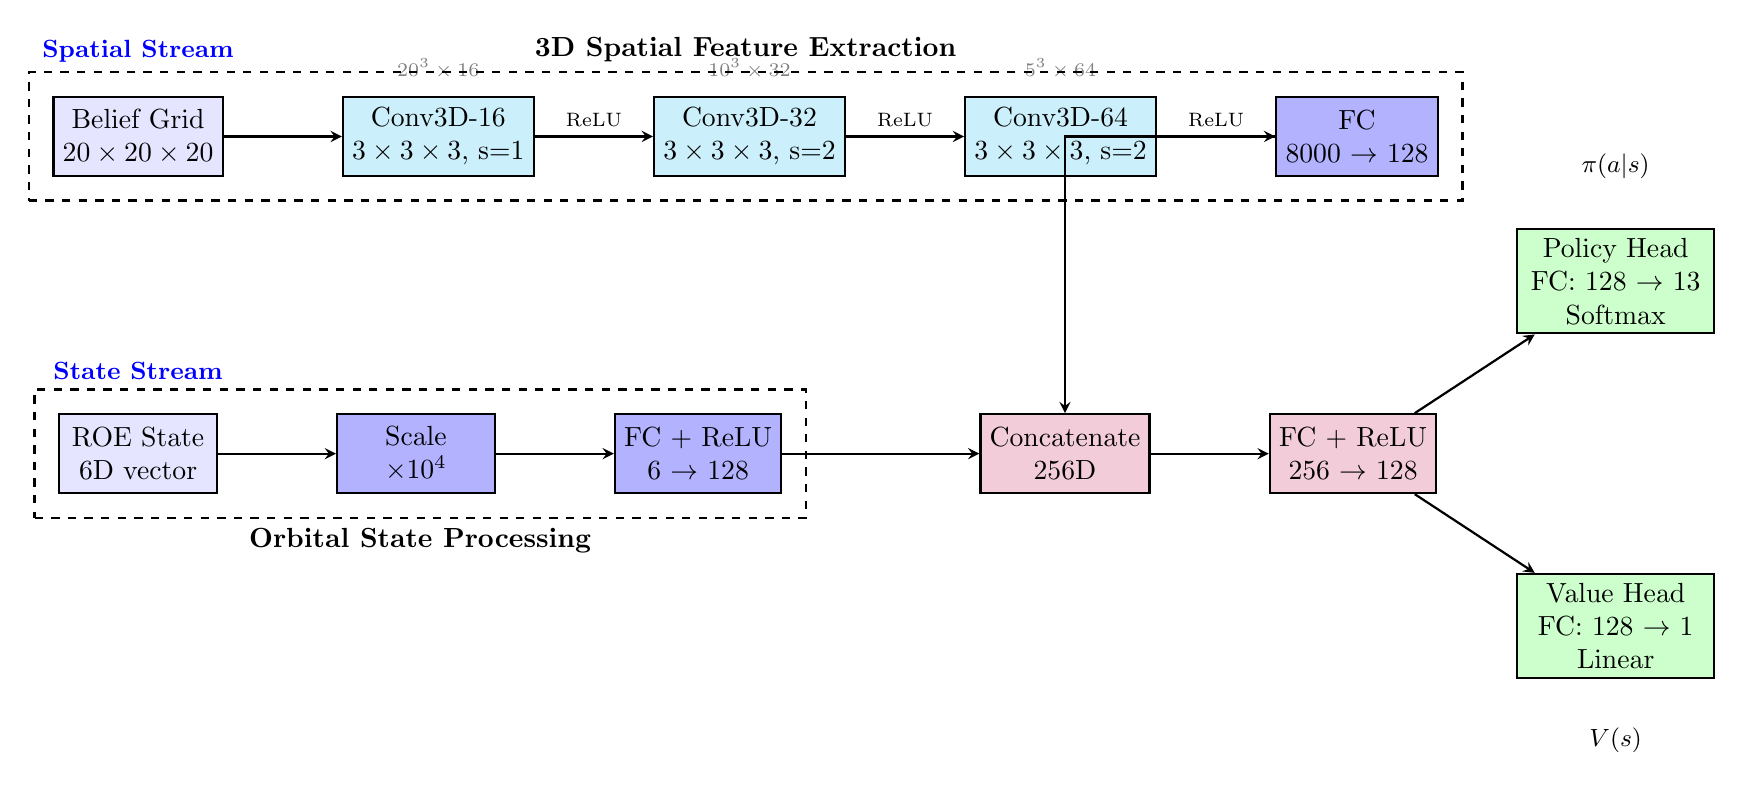
\begin{tikzpicture}[
    node distance=1.5cm,
    box/.style={rectangle, draw, thick, minimum width=2cm, minimum height=1cm, align=center},
    input/.style={box, fill=blue!10},
    conv/.style={box, fill=cyan!20},
    fc/.style={box, fill=blue!30},
    shared/.style={box, fill=purple!20},
    output/.style={box, fill=green!20, minimum width=2.5cm},
    arrow/.style={->, >=stealth, thick}
]

% Belief Grid Stream (Top)
\node[input] (grid_input) {Belief Grid\\$20 \times 20 \times 20$};
\node[conv, right=of grid_input] (conv1) {Conv3D-16\\$3 \times 3 \times 3$, s=1};
\node[conv, right=of conv1] (conv2) {Conv3D-32\\$3 \times 3 \times 3$, s=2};
\node[conv, right=of conv2] (conv3) {Conv3D-64\\$3 \times 3 \times 3$, s=2};
\node[fc, right=of conv3] (fc_grid) {FC\\8000 $\rightarrow$ 128};

% ROE Stream (Bottom)
\node[input, below=3cm of grid_input] (roe_input) {ROE State\\6D vector};
\node[fc, right=of roe_input] (scale) {Scale\\$\times 10^4$};
\node[fc, right=of scale] (fc_roe) {FC + ReLU\\6 $\rightarrow$ 128};

% Shared layers
\node[shared, right=2.5cm of fc_roe] (concat) {Concatenate\\256D};
\node[shared, right=of concat] (fc_shared) {FC + ReLU\\256 $\rightarrow$ 128};

% Output heads
\node[output, above right=1cm and 1cm of fc_shared] (policy) {Policy Head\\FC: 128 $\rightarrow$ 13\\Softmax};
\node[output, below right=1cm and 1cm of fc_shared] (value) {Value Head\\FC: 128 $\rightarrow$ 1\\Linear};

% Arrows - Grid stream
\draw[arrow] (grid_input) -- (conv1);
\draw[arrow] (conv1) -- node[above, font=\scriptsize] {ReLU} (conv2);
\draw[arrow] (conv2) -- node[above, font=\scriptsize] {ReLU} (conv3);
\draw[arrow] (conv3) -- node[above, font=\scriptsize] {ReLU} (fc_grid);

% Arrows - ROE stream
\draw[arrow] (roe_input) -- (scale);
\draw[arrow] (scale) -- (fc_roe);

% Arrows - Convergence
\draw[arrow] (fc_grid) -| (concat);
\draw[arrow] (fc_roe) -- (concat);
\draw[arrow] (concat) -- (fc_shared);

% Arrows - Output
\draw[arrow] (fc_shared) -- (policy);
\draw[arrow] (fc_shared) -- (value);

% Dimension annotations
\node[above=0.1cm of conv1, font=\scriptsize, text=gray] {$20^3 \times 16$};
\node[above=0.1cm of conv2, font=\scriptsize, text=gray] {$10^3 \times 32$};
\node[above=0.1cm of conv3, font=\scriptsize, text=gray] {$5^3 \times 64$};

% Stream labels
\node[above=0.3cm of grid_input, font=\small\bfseries, text=blue] {Spatial Stream};
\node[above=0.3cm of roe_input, font=\small\bfseries, text=blue] {State Stream};

% Final outputs
\node[above=0.5cm of policy, font=\small] {$\pi(a|s)$};
\node[below=0.5cm of value, font=\small] {$V(s)$};

% Add bounding boxes for clarity
\node[draw, dashed, thick, fit=(grid_input) (conv1) (conv2) (conv3) (fc_grid),
      label=above:{\textbf{3D Spatial Feature Extraction}}, inner sep=0.3cm] {};
\node[draw, dashed, thick, fit=(roe_input) (scale) (fc_roe),
      label=below:{\textbf{Orbital State Processing}}, inner sep=0.3cm] {};

\end{tikzpicture}
}
\caption{AlphaZero Policy-Value Network Architecture}
\label{fig:network_architecture}
\end{figure}

\section{Experiments and Results}
\label{sec:results}
%\subsection{Standard MCTS Planner}
%We conducted experiments to validate the efficacy of the MCTS planner in the orbital environment. The servicer was initialized in a standard inspection orbit relative to the target. The simulation parameters and justification for their values is provided in Appendix \ref{appendix:sim}.
%\subsubsection{Entropy Reduction}
%The primary metric for success is the reduction of belief entropy over time. Figure 1 (referencing the internal project figures) demonstrates the progression of total entropy over a 5-step episode. We observed a consistent monotonic decrease in entropy from an initial value of approximately 5550 nats to under 5000 nats. This confirms that the MCTS planner successfully selects maneuvers that reveal previously occluded faces of the RSO, thereby driving the voxel probabilities toward 0 (empty) or 1 (occupied).
%\subsubsection{Trajectory Analysis}
%Qualitative analysis of the trajectory shows that the agent does not simply drift passively. Instead, it executes burns that alter the relative geometry, specifically moving out of the orbital plane (Normal burns) to inspect the "top" and "bottom" of the target, which are typically unobservable in a planar fly-around. The visualization of the ray-casting interactions confirms that the agent prioritizes viewing angles that intersect with voxels holding high uncertainty ($P \approx 0.5$).
%\subsubsection{Discussion}
%The preliminary results indicate that the reward formulation effectively captures the objective of the mission. The trade-off between fuel cost and information gain prevents the agent from making prohibitively expensive maneuvers for marginal information return. While the current MCTS implementation serves as a strong baseline, the computational cost of running ray-casting simulations during the tree search is high. This justifies the proposed transition to the neural network policy, which will distill the MCTS capabilities into a fast forward-pass inference model suitable for real-time onboard deployment.
\subsubsection{MCTS Hyperparameter Tuning}

Hyperparameter sweeps validate MCTS performance using entropy reduction $(H_{\text{initial}} - H_{\text{final}})/H_{\text{initial}} \times 100$ and total $\Delta v$ (m/s) as metrics. Experiments swept horizon $h \in \{10, 15, 20\}$, exploration $c \in \{1.4, 2.0, 3.0\}$, discount $\gamma \in \{0.9, 0.95, 0.99\}$, and fuel penalty $\lambda_{\Delta v} \in \{0.01, 0.1, 0.5, 1.0, 5.0\}$ across 500 and 1000 MCTS iterations. Table \ref{tab:mcts_results} depicts the simulation parameters used for the top performers out of a total of 22 sweeps.

\begin{table}[h]
\centering
\caption{MCTS hyperparameter sweep}
\begin{tabular}{ccccccc}
\toprule
\textbf{c} & \textbf{h} & $\boldsymbol{\gamma}$ & $\boldsymbol{\lambda_{\Delta v}}$ & \textbf{Iters} & \textbf{Ent. Red. (\%)} & \textbf{$\Delta v$ (m/s)} \\
\midrule
1.4 & 15 & 0.99 & 1.0  & 1000 & \textbf{96.77} & \textbf{0.31} \\
1.4 & 20 & 0.99 & 0.01 & 500 & 96.60 & 0.75 \\
1.4 & 20 & 0.99 & 0.1  & 500 & 96.58 & 0.79 \\
3.0 & 10 & 0.99 & 0.5  & 1000 & 96.37 & 1.10 \\
3.0 & 10 & 0.99 & 1.0  & 1000 & 94.96 & 1.17 \\
\bottomrule
\end{tabular}
\label{tab:mcts_results}
\end{table}

Experiments reveal a fundamental tradeoff between planning depth and exploration breadth. Deep planning ($h=20$) achieves $\approx 96.6\%$ reconstruction using only 0.75 m/s, while shallow planning ($h=10$) requires aggressive exploration and 1000 iterations to achieve similar performance (96.37\%) but consumes 47\% more fuel (1.10 m/s), demonstrating that lookahead depth is more fuel-efficient than exploration breadth. The best configuration ($c=1.4$, $h=15$, $\gamma=0.99$, $\lambda=1.0$, 1000 iterations) achieves 96.77\% entropy reduction with 0.31 m/s, validating MCTS as a strong baseline for fuel-constrained active sensing.

\subsection{AlphaZero MCTS Planner}

\subsubsection{Simulation Parameters and Neural Network Hyperparameter Tuning}
The AlphaZero MCTS planner hyperparameters were tuned with sweeps similar to the top performing configuration for pure MCTS. Tables \ref{tab:training_config} and \ref{tab:env_config} exhibit a parameter configuration that balances four key considerations: physical realism, computational tractability, learning complexity, and adherence to standard hyperparameter conventions.

After each batch of self-play episodes, the network undergoes 5 training epochs to prevent underfitting while avoiding excessive optimization on a single data batch. The replay buffer maintains 20,000 transitions (approximately 6 full episodes), providing sample diversity for decorrelating batches while keeping the training distribution relatively on-policy.
\begin{table}[htbp]
    \centering
    %--- First Table (Left) ---
    \begin{minipage}[t]{0.48\textwidth}
        \centering
        \caption{Environment Configuration}
        \label{tab:env_config}
        \small
        \resizebox{\textwidth}{!}{% Optional: Resizes table to fit width exactly
        \begin{tabular}{llr}
            \toprule
            \textbf{Category} & \textbf{Parameter} & \textbf{Value} \\
            \midrule
            \multirow{4}{*}{Simulation}
              & Max Horizon & 5 \\
              & Num Steps & 50 \\
              & Time Step (s) & 120.0 \\
              & Num Episodes & 130 \\
            \midrule
            \multirow{5}{*}{Orbit}
              & $\mu_{\text{Earth}}$ (km$^3$/s$^2$) & 398600.4 \\
              & Semi-major $a_{\text{chief}}$ & 7000.0 \\
              & Eccentricity $e_{\text{chief}}$ & 0.001 \\
              & Inclination $i_{\text{chief}}$ & 98.0$^{\circ}$ \\
              & RAAN $\Omega_{\text{chief}}$ & 30.0$^{\circ}$ \\
            \midrule
            \multirow{6}{*}{\shortstack[l]{Initial ROE\\(Nominal\\$\pm$ Bounds)\\$[m]$}}
              & $\delta a$ & $0 \pm 0$ \\
              & $\delta \lambda$ & $200 \pm 20$ \\
              & $\delta e_x$ & $100 \pm 10$ \\
              & $\delta e_y$ & $0 \pm 10$ \\
              & $\delta i_x$ & $50 \pm 10$ \\
              & $\delta i_y$ & $0 \pm 10$ \\
            \bottomrule
        \end{tabular}
        }
    \end{minipage}
    \hfill % Adds flexible space between the tables
    %--- Second Table (Right) ---
    \begin{minipage}[t]{0.48\textwidth}
        \centering
        \caption{Hyperparameters}
        \label{tab:training_config}
        \small
        \resizebox{\textwidth}{!}{% Optional: Resizes table to fit width exactly
        \begin{tabular}{llr}
            \toprule
            \textbf{Category} & \textbf{Parameter} & \textbf{Value} \\
            \midrule
            \multirow{12}{*}{\shortstack[l]{AlphaZero\\Training}}
              & Batch Size & 64 \\
              & Learning Rate & $5 \text{e-}4$ \\
              & MCTS Iterations & 100 \\
              & Epochs/Cycle & 5 \\
              & Replay Buffer & 20000 \\
              & $c_{\text{PUCT}}$ & 1.4 \\
              & Discount $\gamma$ & 0.99 \\
              & Weight Decay & $1 \text{e-}4$ \\
              & Grad Clip Norm & 1.0 \\
              & Optimizer & Adam \\
              & Scheduler & Cosine \\
              & Min LR & $1 \text{e-}5$ \\
            \midrule
            \multirow{1}{*}{Control}
              & $\lambda_{\Delta v}$ (penalty) & 1.0 \\
            \bottomrule
        \end{tabular}
        }
    \end{minipage}
\end{table}

\subsubsection{AlphaZero MCTS Performance}
\begin{figure*}[h]
    \centering
    \begin{subfigure}[t]{0.5\textwidth}
        \centering
        \includegraphics[height=2.2in]{figures/alphazero_mcts_orbit.png}
        \caption{AlphaZero MCTS Agent Orbit}
        \label{fig:AlphaZero_MCTS_Orbit}
    \end{subfigure}%
    ~
    \begin{subfigure}[t]{0.5\textwidth}
        \centering
        \includegraphics[height=2.2in]{figures/baseline_final_frame.png}
        \caption{Passive Agent Orbit Baseline: No Burns}
        \label{fig:passive}
    \end{subfigure}
    \caption{AlphaZero MCTS and Baseline Orbit Comparison}
    \label{output_traj_comparsion}
\end{figure*}

The trained AlphaZero MCTS agent was tested in the simulation and compared against both the pure MCTS planner and the no-burn baseline. Figure \ref{output_traj_comparsion} depicts the servicer orbiting around the target, performing burns, and taking camera observations. The AlphaZero MCTS planner achieves superior performance over all baselines: it executes only 3 small maneuvers ($\Delta v =$ \SI{0.11}{\frac{\meter}{\second}}) over 50 time steps, achieving 97.1\% entropy reduction. In contrast, the optimized pure MCTS baseline (Table \ref{tab:mcts_results}) requires \SI{0.31}{\frac{\meter}{\second}} to achieve 96.77\% reduction, while the passive agent achieves only 95.8\% with no maneuvers. This demonstrates that AlphaZero achieves 0.33\% better reconstruction quality with 65\% less fuel compared to pure MCTS, executing 57\% fewer maneuvers through learned strategic planning. Given that the $\Delta v$ budget of current small passive observer satellites is on the order of \SI{10}{\frac{\meter}{\second}} for basic station-keeping, the AlphaZero MCTS planner provides an exceptionally fuel-efficient trajectory. The results clearly demonstrate that the neural network successfully distills MCTS planning knowledge, enabling real-time decision-making with superior performance over classical planning approaches. 

\begin{figure*}[h]
    \centering
    \begin{subfigure}[t]{0.5\textwidth}
        \centering
        \includegraphics[height=1.55in]{figures/value_loss.png}
        \caption{Value Loss}
        \label{fig:val}
    \end{subfigure}%
    ~ 
    \begin{subfigure}[t]{0.5\textwidth}
        \centering
        \includegraphics[height=1.55in]{figures/policy_loss.png}
        \caption{Policy Loss}
        \label{fig:pol}
    \end{subfigure}
    \caption{AlphaZero MCTS Network Losses}
    \label{loss}
\end{figure*}

As shown in Figure \ref{loss}, the value network demonstrated strong learning with a 89\% reduction in loss, while the policy network remained essentially stagnant with minimal variance early in the training and decreased from there. This rapid convergence suggests the model may have settled into a local optimum early, as the total loss improvement was driven almost entirely by better value predictions rather than refined action strategies. To address this policy stagnation, future runs will adjust hyperparameters such as the network learning rate, MCTS iterations, or the exploration constant to encourage broader state-space exploration. 

\section{Conclusion and Future Work}
\label{sec:conclusion}
We have presented a framework for active characterization of non-cooperative RSO using reinforcement learning. By modeling the problem as a POMDP and utilizing AlphaZero MCTS over a probabilistic voxel grid, we demonstrated that an autonomous agent can plan maneuvers that significantly reduce shape uncertainty. The results validate the superiority of AlphaZero MCTS over classical planning approaches in orbital proximity operations. The AlphaZero agent achieves 97.1\% entropy reduction with only $\Delta v =$ \SI{0.11}{\frac{\meter}{\second}}, outperforming pure MCTS which requires \SI{0.31}{\frac{\meter}{\second}} for 96.77\% reduction—a 65\% fuel savings with better reconstruction quality. The fact that it beat both the pure MCTS baseline and passive agent demonstrates that the neural network has successfully learned to manipulate orbital geometry strategically through self-play training. This fuel efficiency improvement could be the differentiating factor that leads to a successful mission.

Future work will focus on further training of the AlphaZero MCTS planner. This involves generating a large-scale dataset of self-play episodes to train the policy and value networks, thereby replacing the expensive MCTS rollout phase at runtime. Additionally, we plan to increase the fidelity of the simulation by introducing realistic guidance, navigation, and control errors and solar lighting conditions to challenge the robustness of the vision system. Prior to industry adoption, a safety validation algorithm such as reachability analysis to check for collisions prior to burn execution would be introduced. With these refinements, the, planner will be able to make smart maneuvers, react to lighting conditions, drift, or occlusions, and be able to correct a suboptimal initial orbit, shaping AlphaZero MCTS to be a powerful tool for active characterization of non-cooperative RSO and providing capabilities that far surpass current systems on the market.

\section{Contributions}

Following the status update submission, the project was extended beyond the baseline MCTS implementation to include an AlphaZero-inspired reinforcement learning framework. This extension required: (1) design and implementation of a dual-head neural network architecture combining 3D convolutional layers for spatial voxel grid processing with fully-connected layers for orbital state encoding, (2) development of the self-play training infrastructure with PUCT-guided MCTS, experience replay buffers, and policy-value network training, and (3) comprehensive code optimization to reduce training time via GPU acceleration with CUDA, which improved training convergence by 2.9$\times$ per epoch compared to CPU-only training. These implementation and optimization efforts represent more than 30 hours of development work beyond the base MCTS planner established in the status update.

\textbf{Rahul Ayanampudi}: Developed the relative orbital dynamics simulator. Defined the POMDP state/action spaces, probabilistic voxel grid belief, ray-casting sensor observation model, and reward function. Structured the neural network, parallelized episodes, and trained the network.

\textbf{Sebastian Martinez}: Configured the reinforcement learning problem formulation. Implemented the standard MCTS logic, integrated the planning algorithm with the environment, and performed hyperparameter tuning. Created the AlphaZero-inspired MCTS framework.

The Github repository can be found in \href{https://github.com/rayanam2021/CS229_Final_Project}{https://github.com/rayanam2021/CS229\_Final\_Project}

\bibliographystyle{plainnat}
\bibliography{references}

\end{document}